\Tsubsection{UI1 Sitio} 

\begin{large}
  \textbf{Objetivo}\\\\
\end{large}


Permite al usuario seleccionar la  sección a consultar ya sea \textbf{Política}, \textbf{Deportes}, \textbf{Ciencia y técnología}, \textbf{Economía}
o \textbf{Cultura} y de ser necesario, permite cambiar el periodo de consulta en un rango de 3 días.\\

	

\begin{large}
  \textbf{Descripción}\\\\
\end{large}

La pantalla muestra un menú con las secciones definidas para el sistema, en ella se puede navegar para acceder a las consultas de las noticias clasificadas y de ser necesario, ingresar al sitio web del artículo.\\

%\Large{\textbf{Comandos}}\\
%\normalsize{}
%
%\begin{itemize}
%	\item Lorem ipsum
%	\item Lorem ipsum
%	\item Lorem ipsum
%\end{itemize}


\begin{large}
  \textbf{Referenciado por:}\\\\
\end{large}
\normalsize{\Tref{CU1}{CU1 Recolectar noticias},\Tref{CU4}{CU4 Mostrar resultados}}
%-----------------------------UI1--------------------------%
\begin{figure}[H]\Tlabel{UI1}
  \centering
	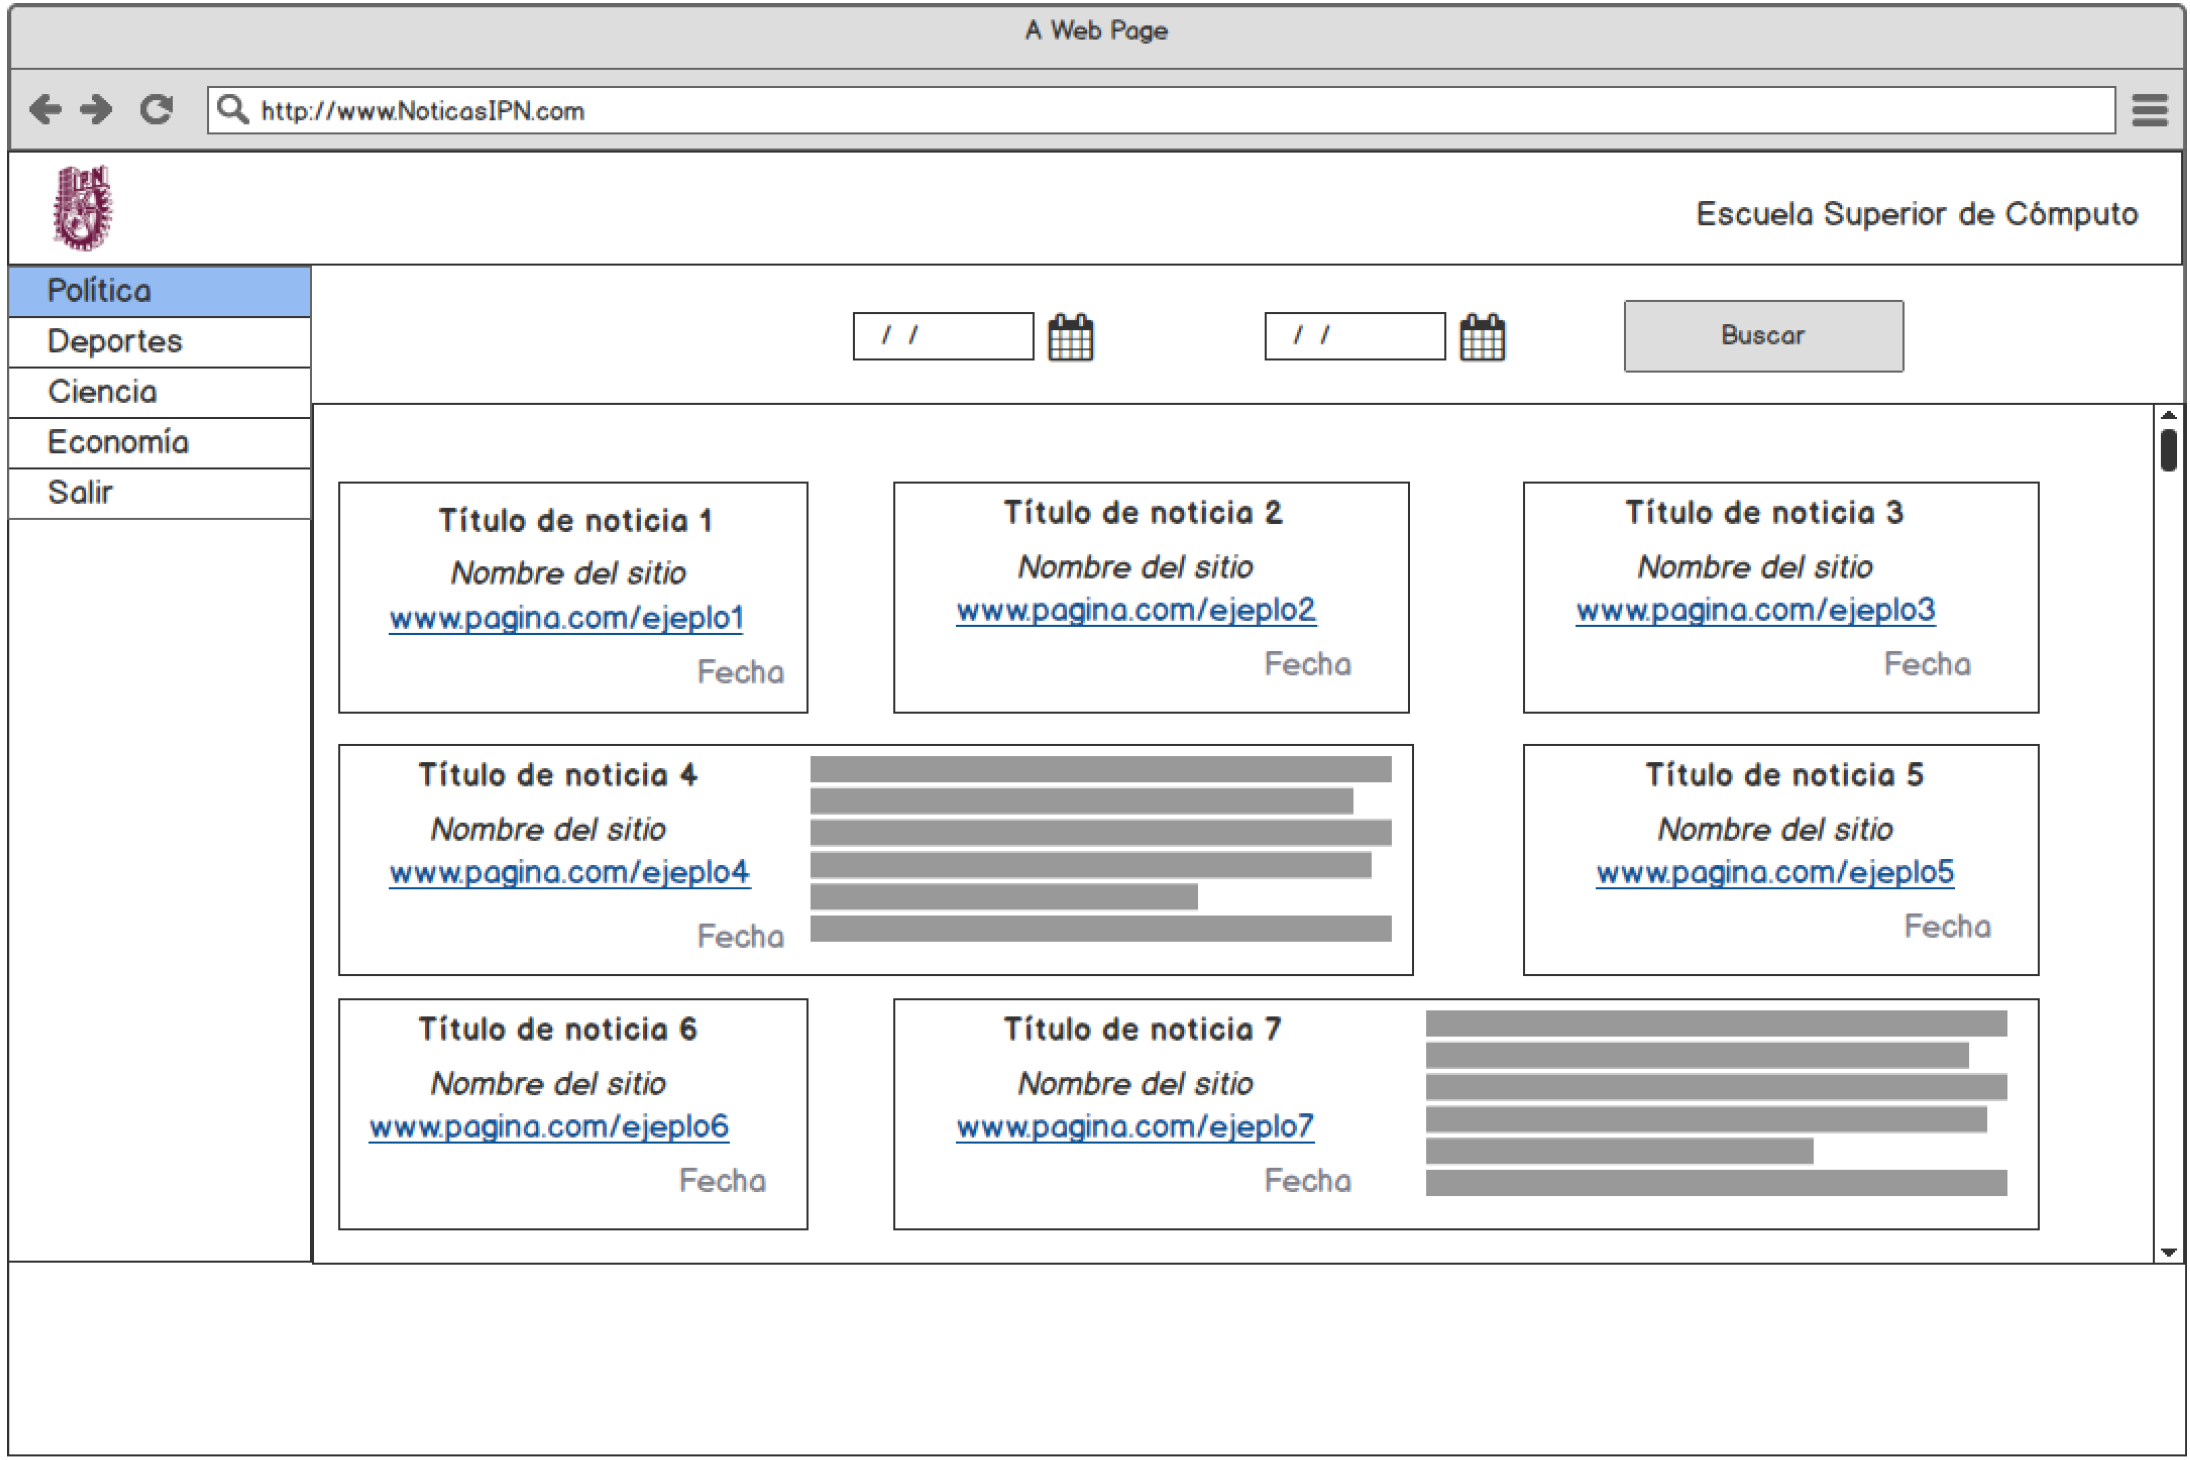
\includegraphics[scale=.35]{imagenes/Pantallas/UI1}
  \caption{Pantalla UI1 Inico}
  \label{fig:UI1}
\end{figure}


%-----------------------------UI2--------------------------%
\begin{figure}[H]\Tlabel{UI2}
  \centering 
	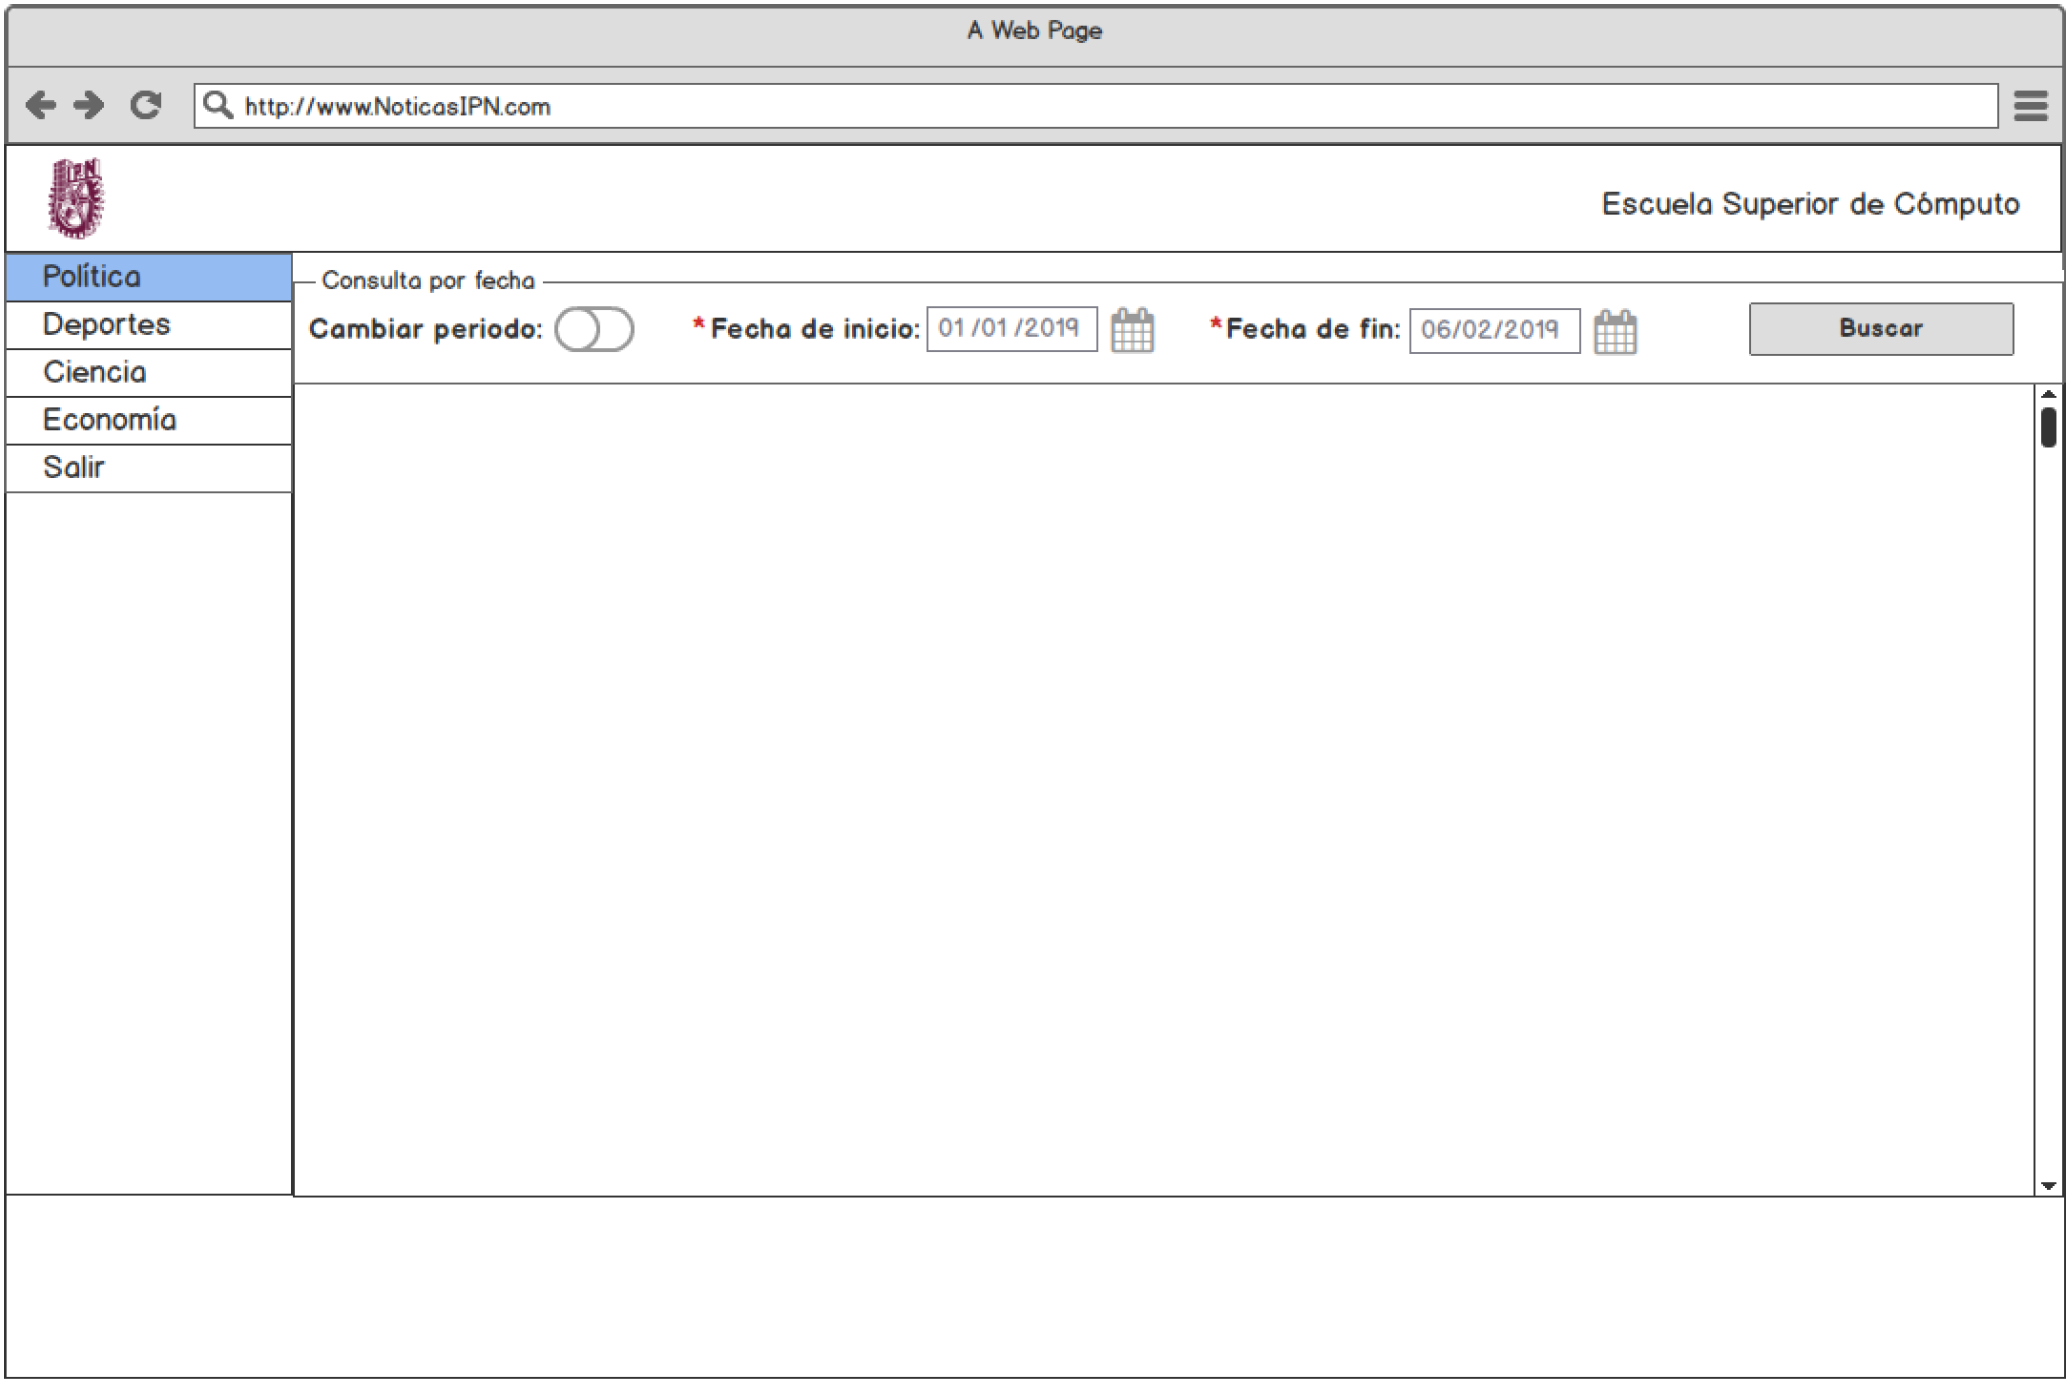
\includegraphics[scale=.35]{imagenes/Pantallas/UI2}
  \caption{Pantalla UI2 Espera de proceso}
  \label{fig:UI2}
\end{figure}

%-----------------------------UI3--------------------------%
\begin{figure}[H]\Tlabel{UI3}
  \centering
	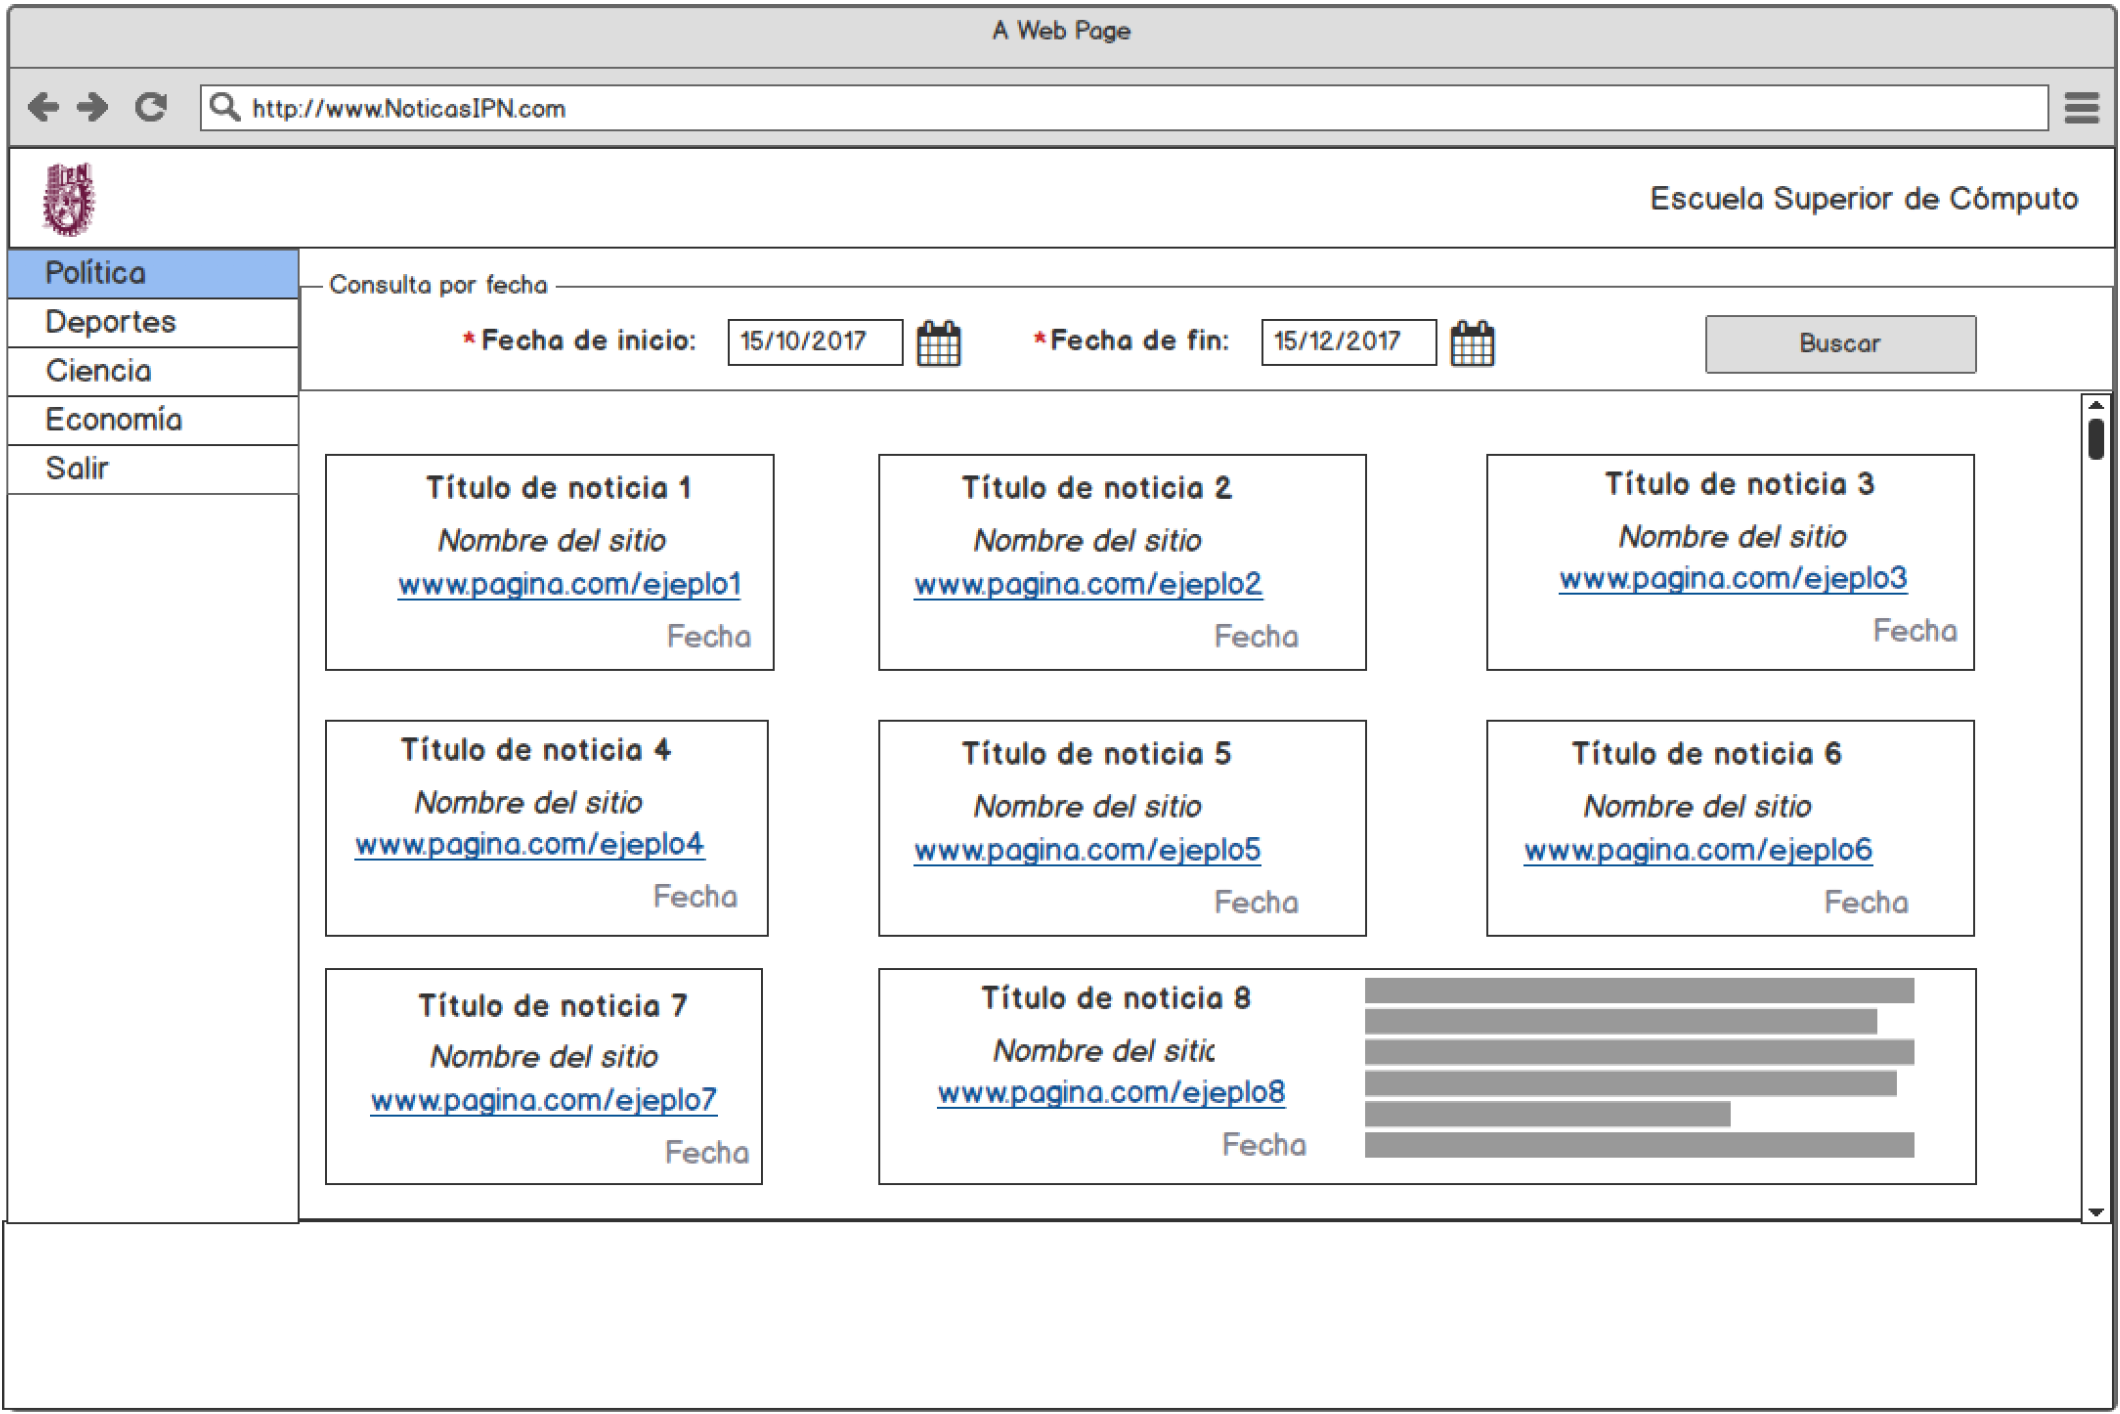
\includegraphics[scale=.35]{imagenes/Pantallas/UI3}
  \caption{Pantalla UI3 Proceso concluido}
  \label{fig:UI3}
\end{figure}
%-----------------------------UI4--------------------------%
\begin{figure}[H]\Tlabel{UI4}
  \centering
  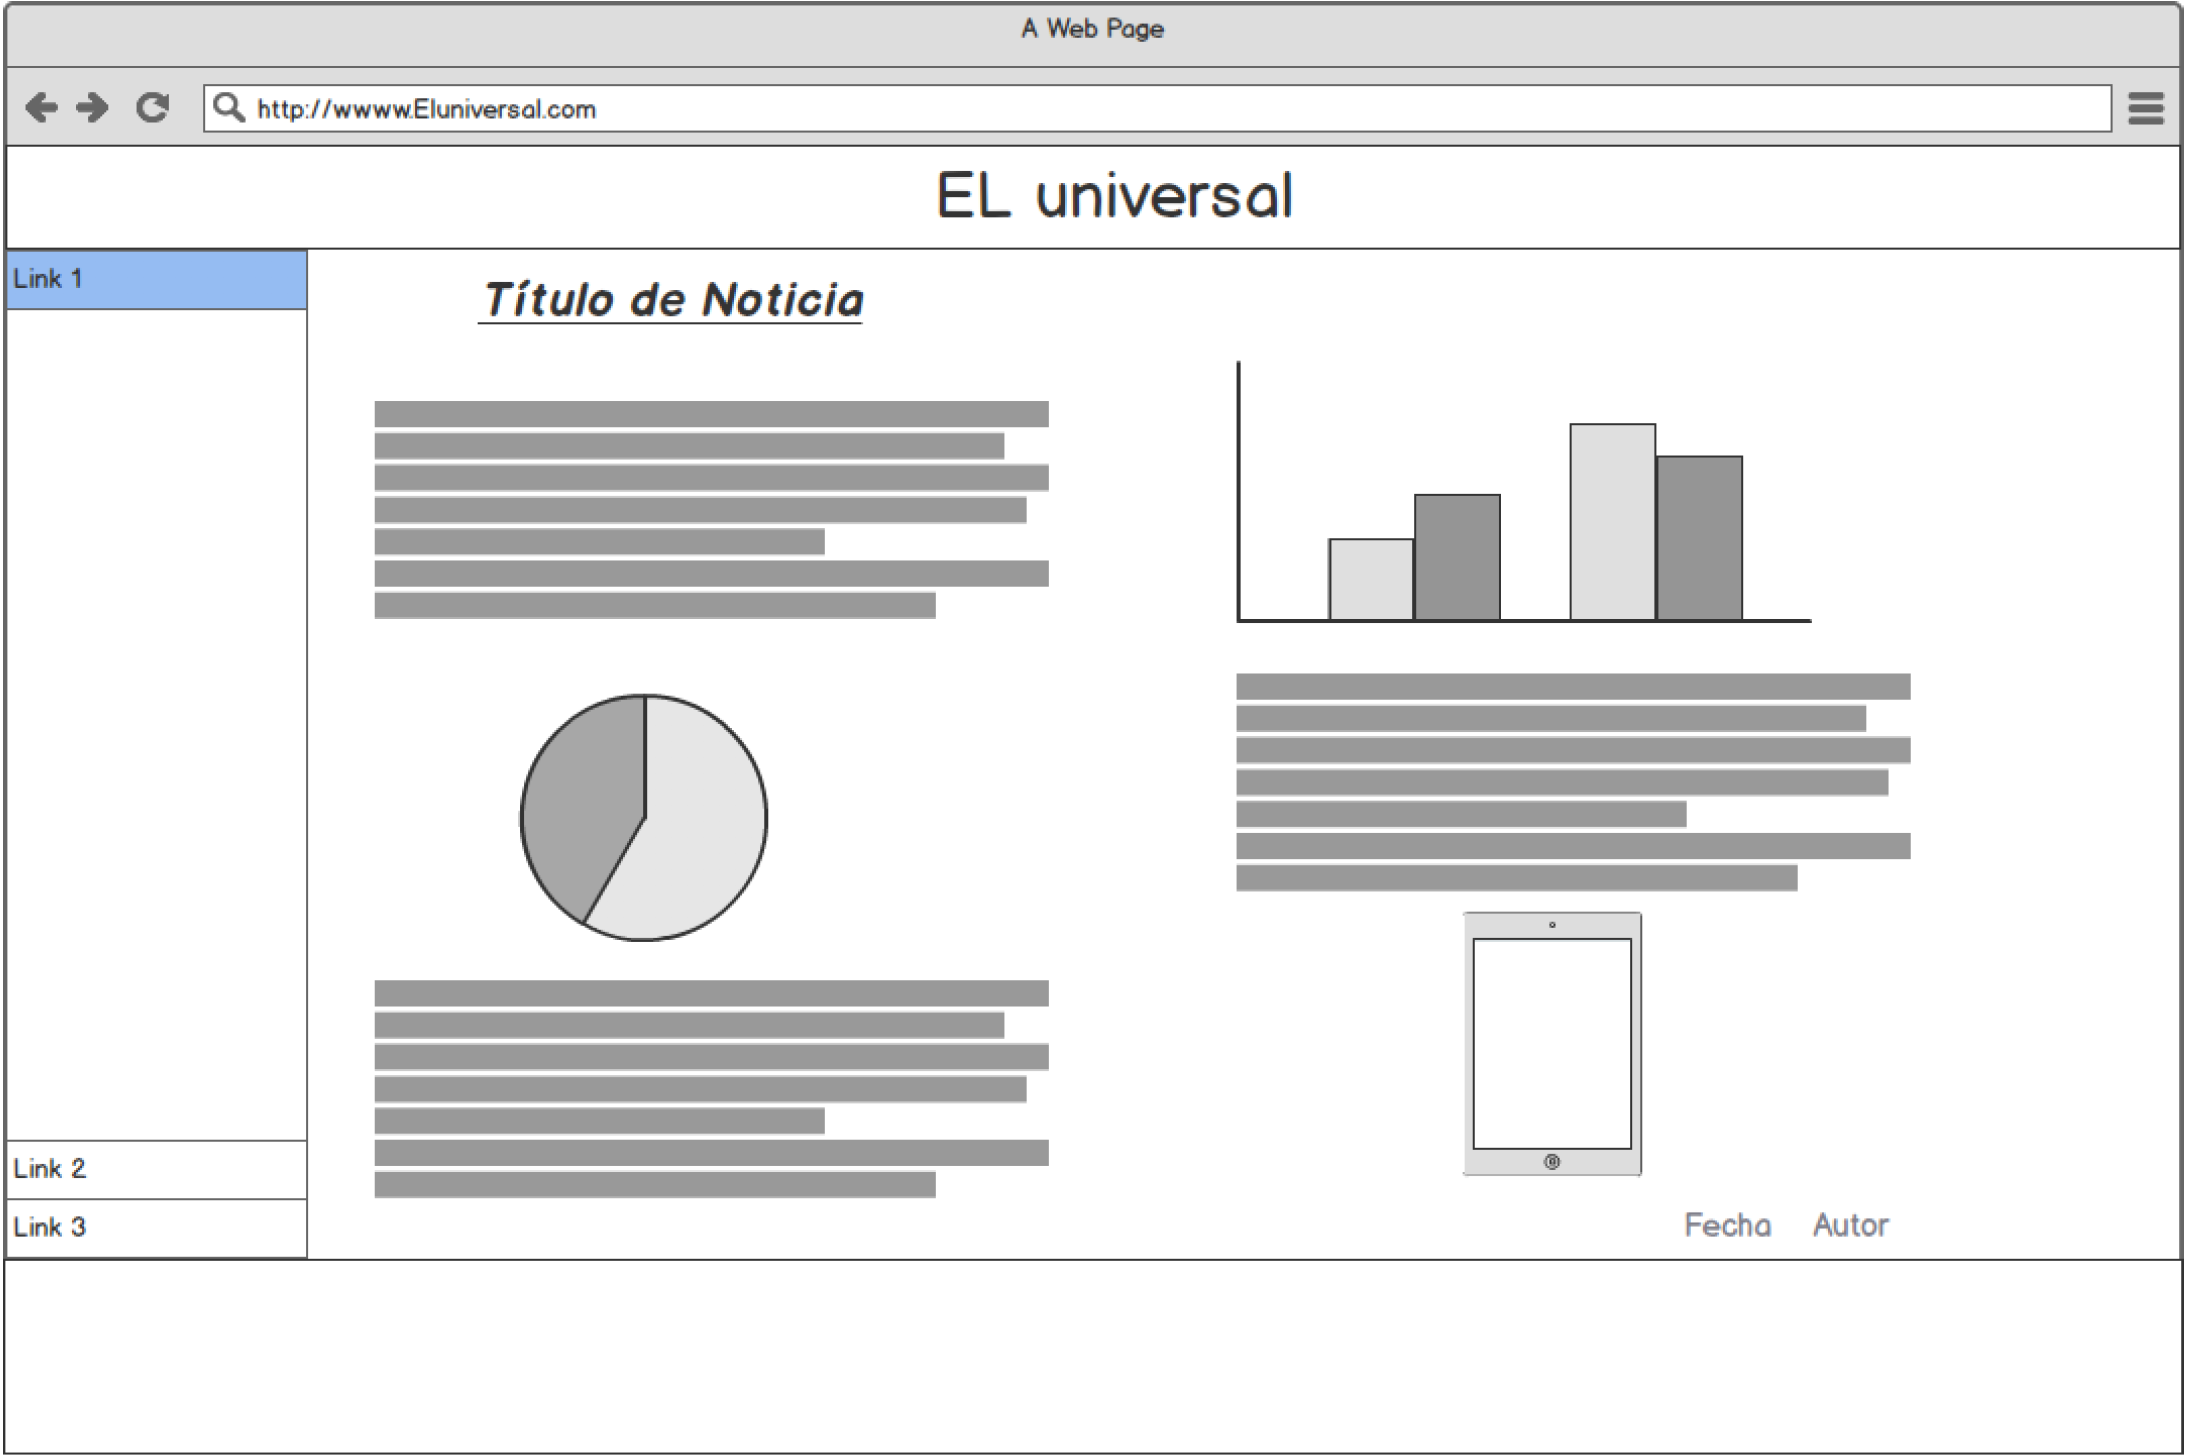
\includegraphics[scale=.35]{imagenes/Pantallas/UI4}
  \caption{Pantalla UI4 Sección polítca}
  \label{fig:UI4}
\end{figure}
%-----------------------------UI5--------------------------%
\begin{figure}[H]\Tlabel{UI5}
  \centering
  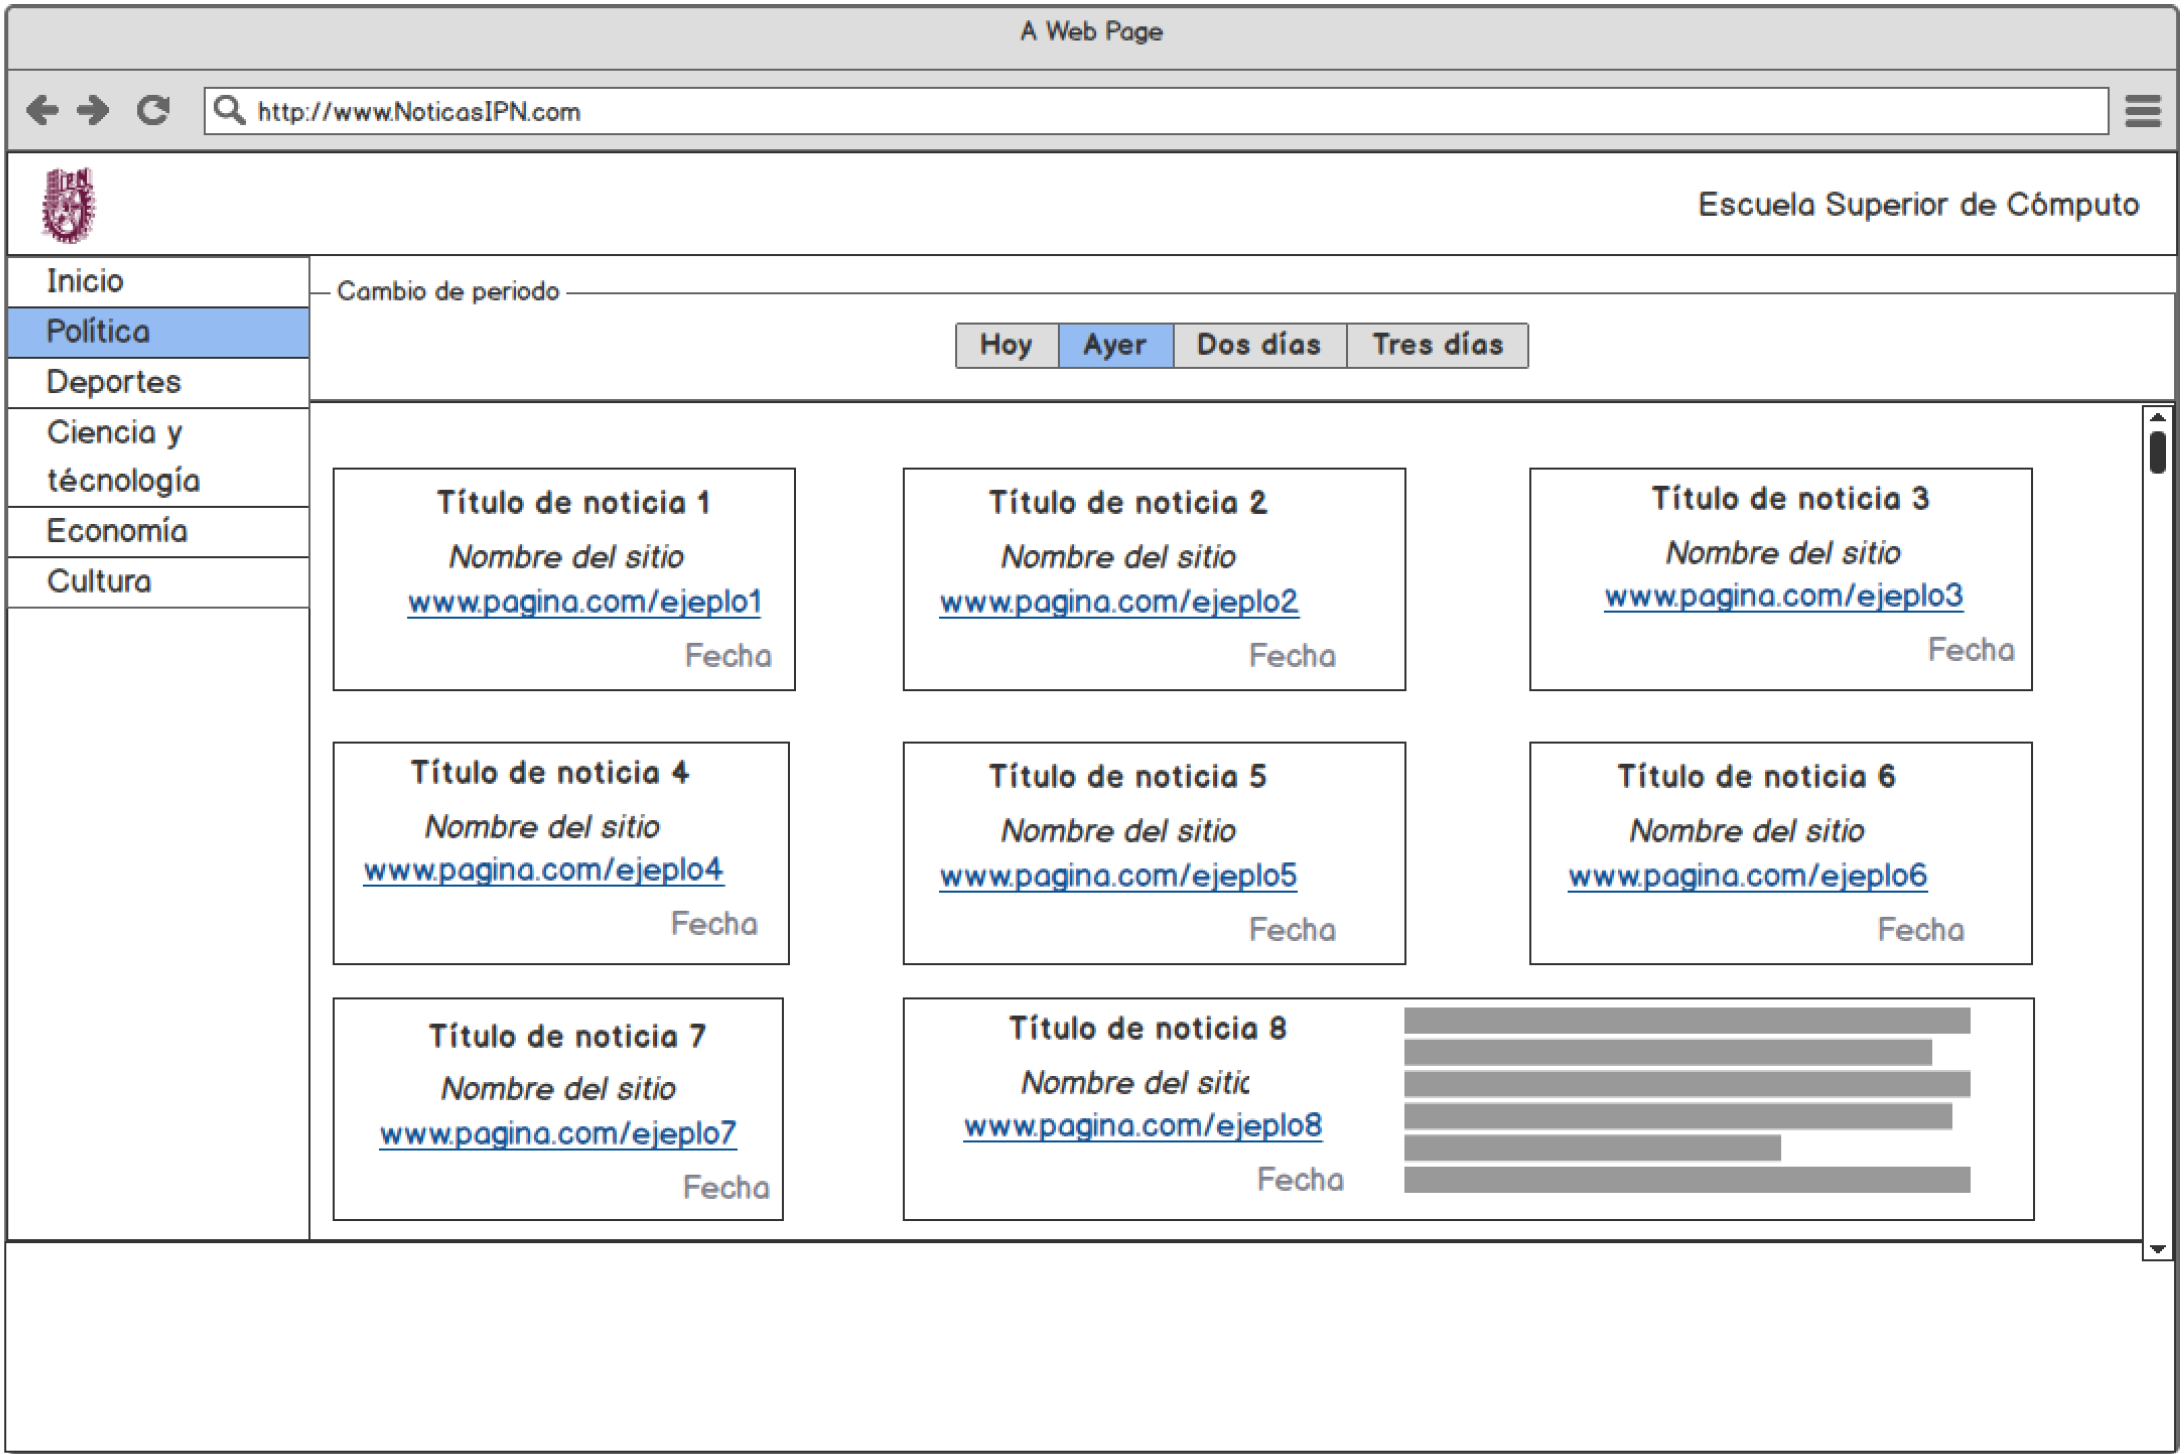
\includegraphics[scale=.35]{imagenes/Pantallas/UI5}
  \caption{Pantalla UI5 Cambio de perido}
  \label{fig:UI5}
\end{figure}

%-----------------------------UI6--------------------------%
\begin{figure}[H]\Tlabel{UI6}
  \centering
	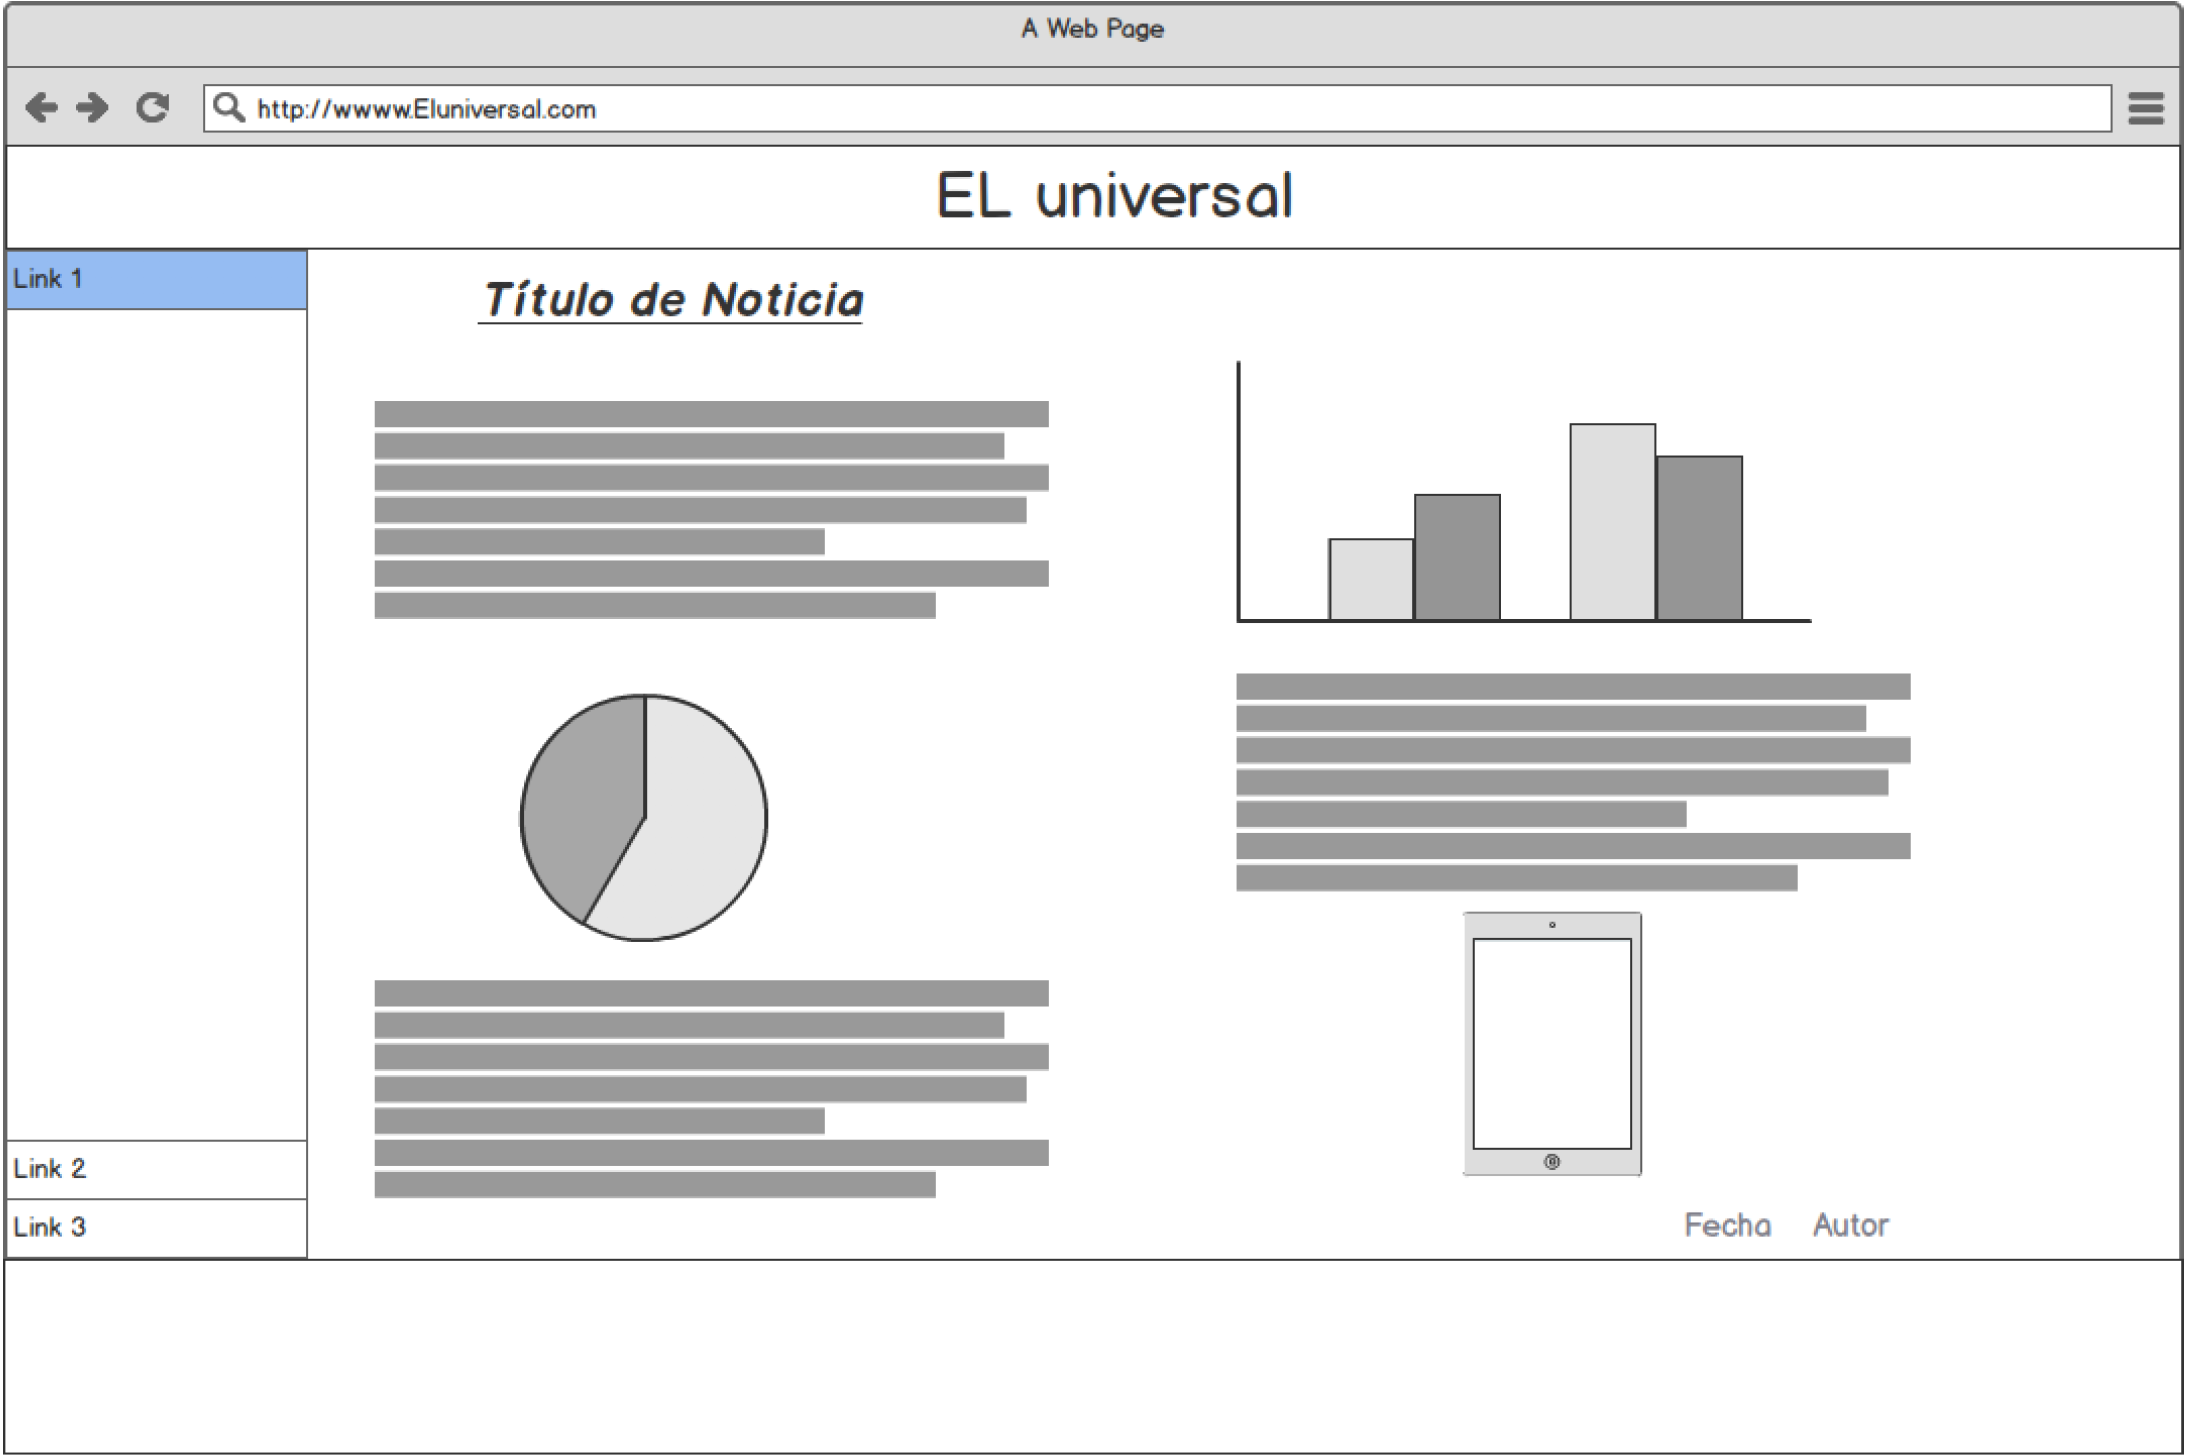
\includegraphics[scale=.35]{imagenes/Pantallas/UI6}
  \caption{Pantalla UI6 Página de sitio web}
  \label{fig:UI6}
\end{figure}